\chapter{Background}

\section{Definitions}
\subsection{Epidemic and Pandemic }
An infectious disease is a disease that is caused by pathogenic microorganisms, such as bacteria, viruses, parasites or fungi; these diseases can be spread, directly or indirectly, from one person to another. An epidemic is a situation where an infectious disease is affecting many people at a particular time and spread at a very high rate. A pandemic on the other hand
is an epidemic over a large area \citep{morens2009pandemic}.

\subsection{Deterministic and Stochastic Infectious Disease Models}
The dynamics of infectious disease propagation are modelled as a dynamical system. A dynamical system is a system that evolves with time over a state space according to a fixed rule. Thus, let $\mathbb{X}$ be a state space $\mathbb{T}$ set of times and $\mathbb{R}$ rule that specifies how the state evolves with time. the rule is a function  whose domain is $\mathbb{X} \times  \mathbb{T}$ and co-domain $\mathbb{X}$ that is,
\begin{equation*}
\mathbb{R}: \mathbb{X}  \times \mathbb{T} \longrightarrow \mathbb{X}.
\end{equation*}

This means that $\mathbb{R}$ takes two arguments $ (\textbf{x},t)$ where $\textbf{x} \in \mathbb{X}$ is the initial state and $t \in \mathbb{T}$. That is $\mathbb{R} (\textbf{x},t)$ gives the state of the system at time $t$ given the initial state of the system was $\textbf{x}$ \citep{DQ}.

\Jnote{It feels to me you are contradicting yourself. If you assume
  continuous time, I don't think it is accurate to represent the disease
  evolution as ``rule'' $\mathbb{R}$. may need your help in this}
The population can be partitioned into different disease states and the movement of individuals from one state to another is tracked over time. Compartmental models are built to tract the flow of individuals in each state at time $t$.


The SIS model, are built to model disease transmission in the case were the population has only two compartments susceptible and infected.The number of people susceptible  at time $t$ is denoted by $S(t)$ and that of infected people is denoted by $I(t)$. The SIS model assumes that there is no immunity after recovery. It is used to model infections were once a person recovers from the infection, they become susceptible again. An example of such an infections disease is flu.

If people have immunity after an infection another compartment $R(t)$, for the number revered people people who recover is added to the SI model. This leads to Susceptible, Infected and Recovered SIR models.For example a person who recovers from Chickenpox develops immunity against it. 

In the case where there is a latent period between when one gets infected and when they become infectious. An intermediate compartment for the number of people who are exposed $E(t)$ is added to the SIR model to make a susceptible, exposed infected and recovered (SEIR) model. An example 

The independent variable in the compartmental models is the time $t$.The rates of transfer between compartments are expressed mathematically as a result models are formulated initially as differential equations. Most epidemic models are built on the SIR model \citep{m1925applications}. The system can be written as;

\begin{align}\label{eqn1_1}
\frac{dS}{dt} &= -\alpha S(t) I(t), \nonumber  \\
\frac{dI}{dt} &= \alpha S(t) I(t) - \gamma  I(t), \\
\frac{dR}{dt} &= \gamma  I(t), \nonumber  
\end{align}
where , $\alpha$ and $\gamma$ are parameters of the model and with assumptions that there is homogeneous mixing in the population. That is the rate of new infections is proportional to the current numbers of susceptibles and infectives in the population. This is the main assumption deterministic models are built on. Deterministic population  models are models where the behaviour of the population of determined completely by history and the rules which govern the model. 

In formulating these models, in terms of derivatives of the sizes of the compartments it is assumed that the number of members in each compartment is differentiable with time. This assumption is tenable only when the disease outbreak has been established, but not valid at the beginning of a disease outbreak, when they are few infectives. When they are a few infectives, the number of infectious depends on random contacts of between a small number of individuals \citep{brauer2012mathematical}.
 
On the other hand, life phenomena are in general stochastic in nature and the dynamics cannot be well captured by deterministic models hence a need
for stochastic models. Stochastic models take into account random variations associated with environmental and biological fluctuations of the factors that affect disease propagation. These random fluctuations may impact the evolution of the infection. Unlike deterministic models which assume homogeneous mix, an assumption which only holds in small populations. It is quite unlikely that all people will be equally susceptible to the disease and effective in spreading it \citep{ball1985deterministic}.

  There are a number of different stochastic modelling processes, such as discrete time Markov chain model, continuous time Markov chain models and stochastic differential equation models. These models differ in underlying assumptions regarding the time and variables.
 
  For example, let us take an SIR compartmental model. S, I and R represent compartments as well as the number of individuals in each compartment and we assume that $S (t) + I (t) + R (t) = N $ is constant. Time $t>0$ is continuous for each state $S (t) $, $I (t) $ and $R (t) $.
  Let $\beta$ to be the average number of contacts an infectious person makes per unit of time that take leads to infection. The probability of a susceptible individual moving from compartment S to compartment I in the time interval $\left[ t,\triangle t \right]$ that is S $\rightarrow S-1$ and I $\rightarrow I + 1 $ is $ \beta$ S I $ \triangle t + o (\triangle t) $.
  \Jnote{I think you should normalize by $N$ here.}
  Assuming that an infected person recovers at the rate $\gamma$ hence the probability of an infected person moving from infected to recovered over an interval $\left[ t,\triangle t \right]$  is given by $\gamma I_ {t + \triangle t} -o (\triangle t) $. Since,
 \begin{align*}
  R(t) = N(t) - S(t) - I(t),
\end{align*}  
which implies that knowing $S(t),I(t)$ is knowing $R(t)$. Hence the model becomes an $S(t),I(t)$ model and thus the stochastic dynamical system can be written as;
 \begin{align}
 P((S(t + \triangle t), I(t + \triangle t) - (S(t) ,I(t)) = (-1,1)) &=  \beta S(t) I(t)  \triangle t + o (\triangle t).
 \\ P ((S(t + \triangle t), I(t + \triangle t) - (S(t) ,I(t)) &= ( 0,-1)) = \gamma I(t + \triangle t) -o (\triangle t).
 \end{align} 
 
With a complementary equation,
\begin{equation}
P((S(t) + \bigtriangleup t, I(t)+ \bigtriangleup t) - S(t), I(t)) =(0,1)) =  -\left( \beta \dfrac{ S(t)}{N}\right) I(t) \bigtriangleup t + o\bigtriangleup t
\end{equation}
\Jnote{Fix typos in equation above.}
which is refereed to as the general stochastic  epidemic model \citep{greenwood2009stochastic}.


\subsection{Network}


A graph also known as a network can be defined as a couple $G = (V, E) $ where $V$ is a finite set of nodes $E \subset V \oplus V = \left\lbrace e_1,e_2,\dots, e_m \right\rbrace$ is a set \citep{estrada2012structure}. Nodes can be human beings, cities or houses while edges could be any connection such as friendship, physical connection or road.

A network is said to be connected if there exists a path between any two nodes in the network. Distance between any two nodes in a network is defined as the length of the shortest path between them.

This can be summed up as the average distance taken over all pairs of vertices, which give the idea of the typical distance between nodes in a network. The diameter of the graph is the largest distance taken over all pairs.

\subsection{Statistical Characterization}
 
Networks can be characterized by the following statistical properties.
 \begin{itemize}
 \item[i] \textit{\textbf{Degree distribution:}}
   The degree of a node is the number of connections to other nodes, a particular node has and is denoted by $k$ and the average degree of a network  of a network is denoted by $\langle k \rangle$. Looking at the entire space or network one can obtain a distribution for the degree. Let $n (k) $ be the number of nodes of degree $k$ in a network of size $n$, $p (k) = \dfrac{n(k)}{n}$. Where $p (k) $ represents the probability that a node selected uniformly at random has degree $k$. The degree distribution is obtained by plotting $p(k)$ against $k$ \citep{estrada2015first}. The common distribution found in the network are normal distribution, exponential, power law distribution and Poisson distribution\citep{chung2002average}.

 \item[ii] \textit{\textbf{Clustering: }}
   A cluster in a network  is a collection of nodes which are similar among them and are dissimilar to other nodes belonging to other clusters. Clustering in friendship network may signify friends people have in common. Local clustering in a network is measured by  the Watts-Stogatz coefficient and the global clustering by  Newman clustering coefficients.
 
 Watts-Strogatz average clustering coefficient is given by 
 \begin{align}
 \overline{C} = \dfrac{1}{n} \sum_i c_i
  \\ c_i = \dfrac{2t_i}{k_i(k_i-1)} \nonumber
  \end{align}
   where $t_i $ is the number of triangles attached to node $i$ of degree $k_i$. The Watts-Strogatz clustering coefficient of a node quantifies how close its neighbours are close to making a clique. In terms of friends it quantifies how one's friends are friends with each other. The clustering coefficient lies between 0 and 1, if its zero, then no two nodes of a node's neighbours are connected and if it is 1 then all the neighbours of a node are connected to connected to each other.
  

 The Newman clustering coefficient is given by
 \begin{equation}
 c = \frac{3t}{p_2} =\dfrac{3|c_3|}{p_2}
 \end{equation}
 where $t = c_3$ number of triangle in the network and $|p_2|$ the number of closed paths of length 2. 
 The Newman clustering coefficient quantifies how clustered a network is as a whole. Nodes with less than two neighbours are given 0 as the clustering coefficient. 
\end{itemize}

 
In a social network if a person A is friends with person B and B friends with C
it is most likely that A will be introduced to C and the two will know each other. This will result in the three forming a triangle. The clustering coefficient either global or local gives a proportion of how many such triangles are there and how many are likely to exist. The local  clustering coefficient will give this value in relation to a particular node while the global clustering coefficient will give the value over the entire network \citep{estrada2015first}.
 
A network is said to be small world or to exhibit small world properties if its Newman clustering coefficient is greater than the Watts-Strogatz clustering coefficient.
That is a small world network has a high clustering coefficient and a low average distance \citep{estrada2012structure}. A small world property can be defined as let $D$ be the average distance between any pair of vertices in a network, if $D$ increase proportionally to the logarithm of the size of the network$N$ \citep{newman1999scaling}.
  there are multiple definition
That is,
 \begin{equation}
 D \propto \log N
\end{equation}

A high clustering coefficients represents local connectivity and results in near cliques and the short average distance represents global connectivity of nodes in a graph  citep{Mehlhorn2013}.

 
\subsection{Random Graphs} 
A random graph $G(N,p)$ can be defined as , given  $N$ number of vertices, edges between them are drown such that between any pair $i,j$ there is an edge with uncorrelated probability $p$. 

 Let $z$  be the average degree. The probability $p$ of an edge being present between any two vertices is given by $p = \frac{z}{N-1}$, for large N it can be approximated by $\frac{z}{N}$ \citep{newman2002random}. The degree $k$ of a vertex has a probability distribution $p_k$ given by;
 \begin{equation}
 p_k = \binom{N}{k} p^k (1-p)^{N-k} \approx \frac{z^k e^{-z}}{k!},
\end{equation}
for  a constant $k$ and large $N$.

For example, let us take 20 vertices draw  an edge between any vertices with probability $p = 0.2$ We can get a random network shown in
figure
\ref{fig:3.1} below. 
  
  It can be shown that a random graph can exhibit small world effects. Assuming that person A, represents a node on a network such as figure \ref{fig:3.1}. A has $z$ neighbours and about $z^2$, $z^3$ second and third neighbours respectively, and so on. Then the diameter of the network $D$ is given by $z^D = N$. Thus
   \begin{equation*}
D = \frac{\log N}{\log z} 
\end{equation*}
    The logarithmic increase in the diameter of the network and the distance between nodes is typical of a small world effect. Since $\log N$ increases slowly with $N$ it allows the distance to be quite small in very large systems \citep{newman2000models}.  Random networks have a low clustering coefficient $ c = \frac{z}{N}$ \citep{newman2003structure}.
   \begin{figure}[h!]
   \caption{Random Graph with N =20 and p = 0.2}
   \label{fig:3.1}
   \centering
   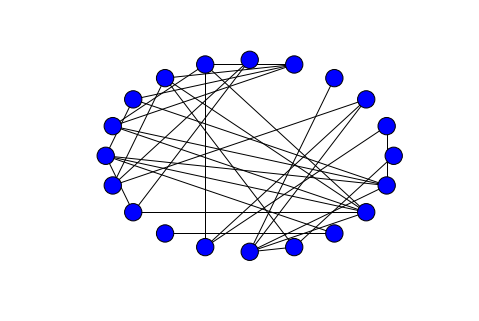
\includegraphics[scale=0.5]{images/randomgraph.png} 
   \end{figure}
   
%
%
%\begin{figure}[h]
%    \centering
%    \begin{subfigure}[b]{0.3\textwidth}
%        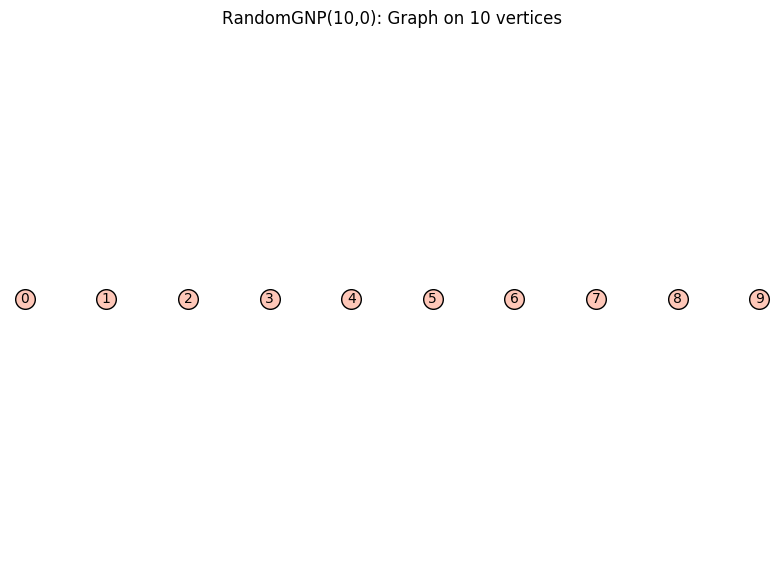
\includegraphics[scale=0.3]{images/rgraph2.png} 
%        \caption{ $p =0$}
%        \label{fig:a}
%    \end{subfigure}
%    ~ %add desired spacing between images, e. g. ~, \quad, \qquad, \hfill etc. 
%      %(or a blank line to force the subfigure onto a new line)
%    \begin{subfigure}[b]{0.3\textwidth}
%        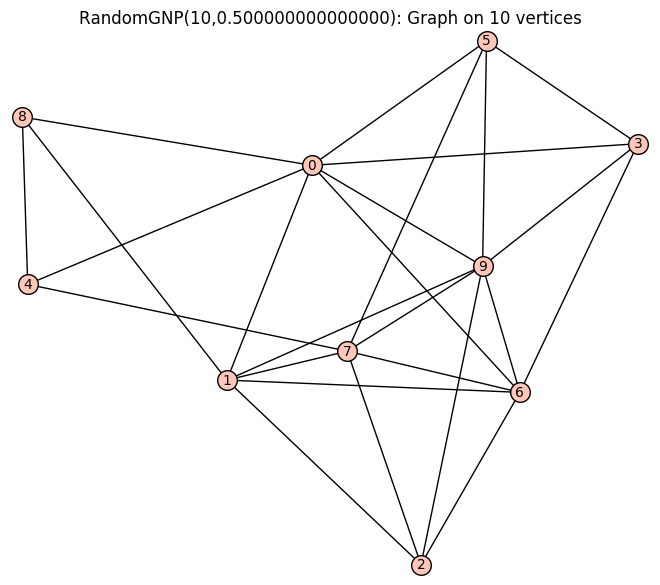
\includegraphics[width=\textwidth]{images/rgraph1.png}
%        \caption{$p=0.5$}
%        \label{fig:b}
%    \end{subfigure}
%    ~ %add desired spacing between images, e. g. ~, \quad, \qquad, \hfill etc. 
%    %(or a blank line to force the subfigure onto a new line)
%    \begin{subfigure}[b]{0.3\textwidth}
%        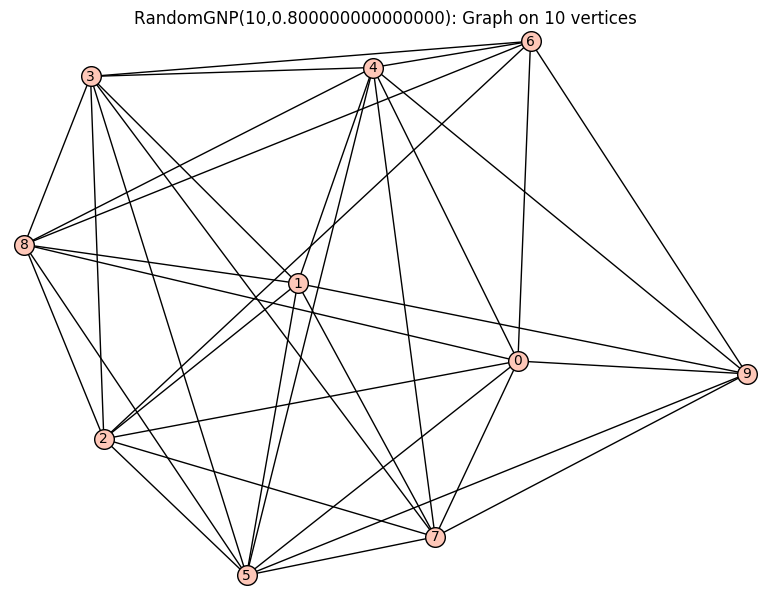
\includegraphics[width=\textwidth]{images/rgraph3}
%        \caption{$p= 0.8$}
%        \label{fig:c}
%    \end{subfigure}
%    \caption{Random Graphs}\label{fig:randomgraphs}
%\end{figure}
%
However,  random  networks  are  not  a  good  model  of  social  networks.  People’s  circles  of  
acquaintances  tend  to  overlap  to  a  great  extent. Random models have a very low clustering coefficient.
\subsection{Ordered Lattice:}
In order to deal with real world networks, graphs must have both high clustering and small world effect properties.Random graphs as discussed earlier show a small world effect. Their  average vertex to vertex distance increase only logarithmically with N but they do not show low clustering \citep{newman2000models}. This leads us to another graph model which is an ordered lattice.

The opposite of a random graph is a completely ordered lattice. An ordered lattice is a graph where each vertex is connected to its $z$ neighbours. A lattice can be drawn in many dimensions. For example, figure \ref{fig2222} shows two lattices drawn in different dimensions.
\begin{figure}[h!]
    \centering
    \begin{subfigure}[b]{0.4\textwidth}
        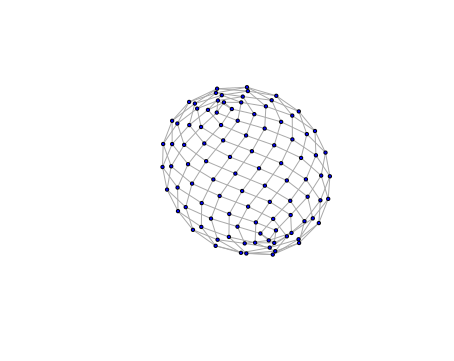
\includegraphics[scale=0.6]{images/lattice1.png} 
        \caption{A square lattice, with $z$ =4}
        \label{fig:gull}
    \end{subfigure}
    ~ %add desired spacing between images, e. g. ~, \quad, \qquad, \hfill etc. 
      %(or a blank line to force the subfigure onto a new line)
    \begin{subfigure}[b]{0.4\textwidth}
        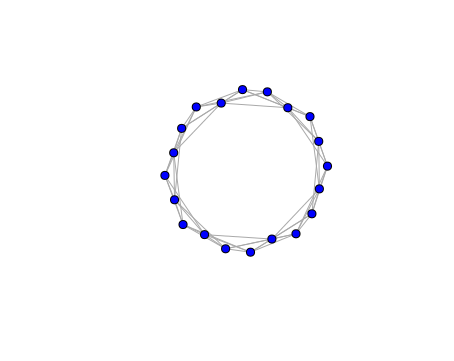
\includegraphics[scale=0.6]{images/ringlattice.png} 
        \caption{A ring lattice, with $z$ = 3}
        \label{fig ring}
    \end{subfigure}
    ~ %add desired spacing between images, e. g. ~, \quad, \qquad, \hfill etc. 
    %(or a blank line to force the subfigure onto a new line)
    \caption{Different types of regular lattices}\label{fig2222}
\end{figure}


Regular lattices and random graphs have a long history of use in network theory and modelling of population structures, \cite{harris1974contact} gives an example of a classic lattice .

The clustering coefficient of a lattice is given as  
\begin{equation}
C = \frac{3(z - d)}{4(z -2)}
\end{equation}
where $d$ is the dimension of the lattice. For a large $z$, $C$ tends to $\dfrac{3}{4}$.

However, regular lattices do not show the small world effect of vertex to vertex distances which increase slowly with size. For a regular lattice of higher dimensions such as the shape of a square or hypercube of size L with $N = L^d$ vertices, the average vertex to vertex distance increases linearly with the system size, which is not typical of the small world behaviour.  


Models built on latices assume that individuals are  nodes on a regular lattice and connections are made of some collection of near neighbours or each node. For example, people may be spread out such that connections are made to their four nearest neighbours, one on the left, right, up and down or  eight neighbours including the four diagonal elements  \citep{lloyd2006infection}.

The main difference between a random graph and lattice is that, in lattice networks interactions are local, that is individuals are only related to their neighbours. Where as in random networks the connections  made are global, that is, connections are made without taking spatial locations of an individual into consideration. 

\subsection{Watts - Strogats Small World Networks}
We have shown that lattices are characterised by high clustering coefficients but long path lengths or vertex to vertex distances. That is, it takes many steps to move between any two randomly selected vertices, whereas random networks have shorter vertex to vertex distances, since there are many long range links, but low clustering \citep{keeling2005networks}.


Small world networks were first introduced by Watts and Strogatz as an intermediate between a regular lattice and a complete graph. They are built by randomly rewiring certain proportions of the network links with a probability $p$ \citep{watts1998collective}. The small world networks allow for random contacts across the network. That is in addition to near neighbours as a regular lattice, each node has a random distant neighbour connected to it \citep{watts1998collective}.


The Watts-Strogatz network is essentially a regular lattice with some degree of randomness in the connectivity of vertices. Take for example in figure \ref{fig ring} above and we rewire some edges with a some probability $p$, that is one of its ends is moved into a randomly chosen position on the lattice. For a small $p$ this produces mostly a regular graph, but with a few connections stretched along distances across the lattice and for $p =1$ it produced a complete graph. Figure \ref{fig } below shows Watts- Strogats networks with different probabilities.

\begin{figure}[h!]
    \centering
    \begin{subfigure}[b]{0.4\textwidth}
        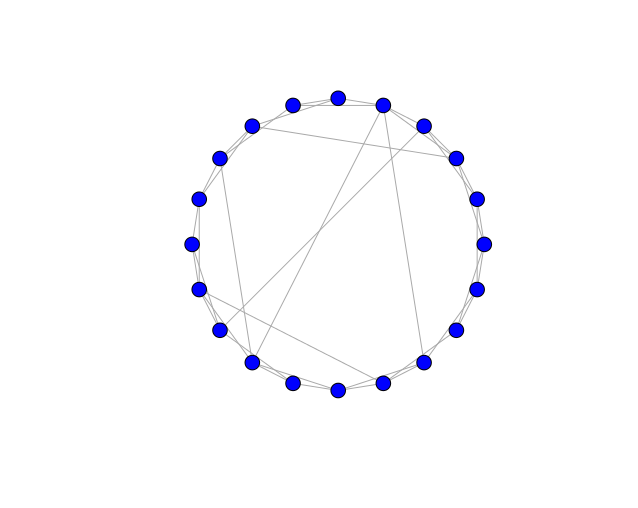
\includegraphics[scale=0.4]{images/sw_p1.png} 
        \caption{A Small world, with $p$ =4}
        \label{fig:gull}
    \end{subfigure}
    ~ %add desired spacing between images, e. g. ~, \quad, \qquad, \hfill etc. 
      %(or a blank line to force the subfigure onto a new line)
    \begin{subfigure}[b]{0.4\textwidth}
        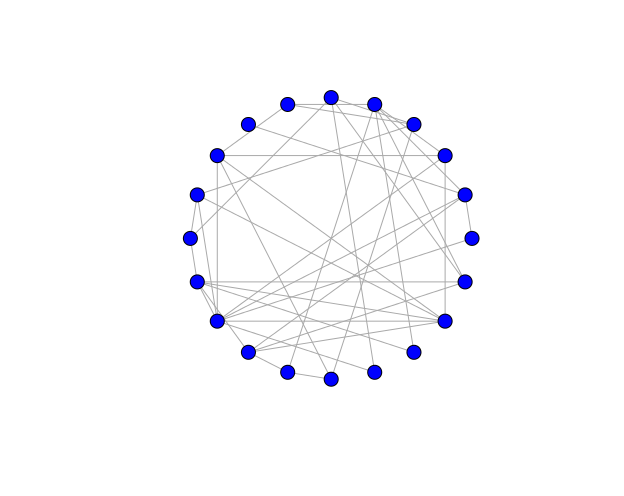
\includegraphics[scale=0.4]{images/sw_p5.png} 
        \caption{A Small world network, with $p$ = 0.5}
        \label{fig }
    \end{subfigure}
    ~ %add desired spacing between images, e. g. ~, \quad, \qquad, \hfill etc. 
    %(or a blank line to force the subfigure onto a new line)
    \begin{subfigure}[b]{0.4\textwidth}
        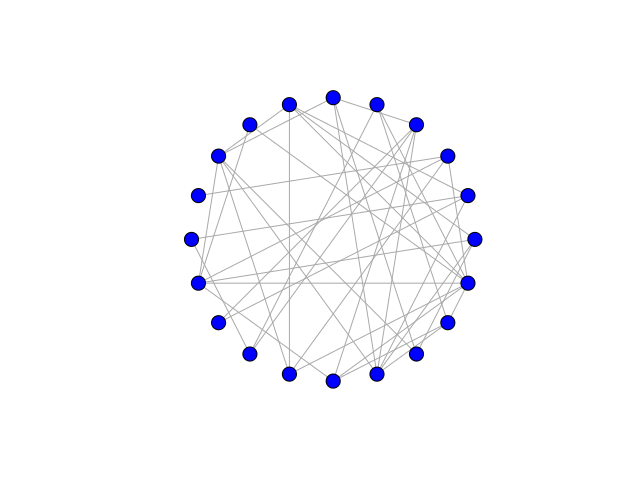
\includegraphics[scale=0.4]{images/sw_p8.png} 
        \caption{A Small world network, with $p$ = 0.8}
        \label{fig }
    \end{subfigure}
    \caption{Watts- Strogatz}\label{fig networks}
\end{figure}
